\section{Vorbereitung}
Vor der Durchführung eines Penetrationstests müssen verschiedenste Aufgaben erledigt und Rahmenbedingungen geklärt werden.

\subsection{Fragebogen}
Um einen ersten Eindruck zu bekommen, was getestet werden soll, empfiehlt sich die Durchsprache eines standardisierten Fragebogens. Im Rahmen dieser Arbeit wurde der Fragebogen von \url{http://www.pentest-standard.org/index.php/Pre-engagement} übersetzt und erweitert.

TODO
\url{http://uweziegenhagen.de/wp-content/uploads/2013/08/LaTeX_and_Python.pdf}

\subsubsection{Implementierung in Latex}
In einem ersten Schritt wurde der Fragebogen übersetzt und um einen allgemeinen Teil ergänzt, welcher dem Pentester bei der Orientierung helfen soll. So werden die verschiedenen Arten von Tests abgefragt und die entsprechend notwendigen Abschnitte genannt.

Zudem wurden die Fragen in Boxen integriert, sowie Ja/Nein-Antworten ansprechend dargestellt. Dies ist in Abbildung \ref{fig:FragLatex} dargestellt. Der Quelltext ist unter \ref{ap:FragTex} im Anhang dargestellt.

\begin{figure}[htbp]
	\centering
	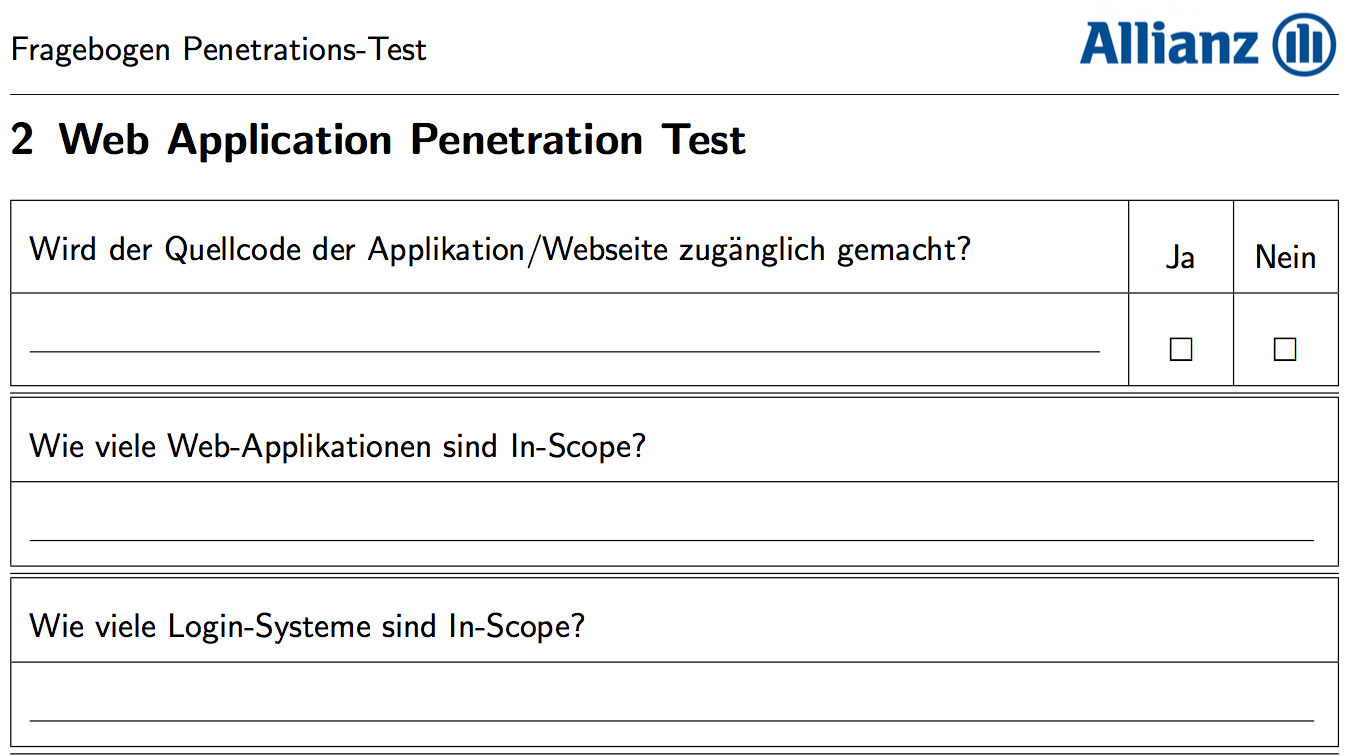
\includegraphics[width=\textwidth]{bilder/pentest_prozesse/vorbereitung/fragebogen_latex.png}
	\caption{Ein kurzer Ausschnitt des Fragebogens mit formatierten Fragen}
	\label{fig:FragLatex}
\end{figure}



\subsubsection{Implementierung als Webabwendung}

\subsubsection{Portierung nach Docker}

	\subsection{Aufwandsschätzung}
	Ein äußert wichtiger aber auch sehr schwieriger Punkt ist die Aufwandsschätzung. Natürlich können klassische Methoden der Aufwandsschätzung aus dem Bereich der Projektmanagement verwendet werden, jedoch müssen eine Vielzahl weitere technischer Aspekte betrachtet werden.
	
	Viele Firmen berechnen den Aufwand aus der Anzahl der Eingabefelder. Leider ist diese Vorgehensweise oft nicht zielführend, da die Komplexität des dahinter liegenden Systems nicht in Betracht gezogen wird. Wird zum Beispiel eine Webseite mit einem Framework erstellt, welches Eingaben stetig Filtert, ist die Wahrscheinlichkeit eine XSS oder SQLi zu finden, relativ gering. In diesem Fall sollte man andere Komponenten wie die Authentisierungslogik oder den Webserver selbst angreifen. Dies würde durch die Aufwandsschätzung rein nach Eingabefeldern nicht in Betracht gezogen.
	
	Blia bla blub mischung.. TODO
		
		
	\subsection{Rechtliche Aspekte}
		\subsubsection{BDSG}
		\subsubsection{NDA}
		\subsubsection{Haftungsausschluss}
		\subsubsection{Absicherung gegen §203STGB}
	\subsection{Technische Aspekte}
		\subsubsection{Infrastruktur}
		\subsubsection{Tools}